\newpage

{%
\footnotesize
\textit{Uwaga: przytoczone fragmenty mogą być luźną interpretacją relacji podanego autora.}
}

\DeclareRobustCommand{\wioslo}{%
  \begingroup\normalfont%
  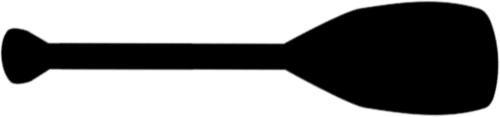
\includegraphics[height=0.8\fontcharht\font`\B]{images/wioslo.png}%
  \endgroup
}

\newcounter{notka}[section]
\newenvironment{notka}[2]{
    \refstepcounter{notka}
    \def\tytul{#1}
    \def\autor{#2}
    \bigskip
    \Large \wioslo{} \hspace{0.2cm} \tytul{}
    \normalsize
    \bigskip

    \begin{adjustwidth}{1cm}{1cm}
}{
    \end{adjustwidth}
    \hfill{} \autor{}
}

\begin{notka}{Śpiewanie na wodzie}{Ola Gawryła}
    Magia mórz, oceanów i innych mniejszych, większych oraz pośrednich
    akwenów wodnych zawierających ciekłe \ce{H2O} powoduje, że każdy
    nagle śpiewa pięknie, nikt nie fałszuje i możemy się tylko
    zachwycać swoimi cudownymi głosami.
\end{notka}

